\documentclass{ctexart}
\usepackage{geometry}
\usepackage{fancyhdr}
\usepackage{graphicx}
\usepackage{booktabs}
\usepackage{multirow}
\usepackage{amsmath}
\usepackage{tikz}
\usepackage{array}
\xeCJKsetup{CJKmath=true}
\usepackage{caption}
\captionsetup{labelformat=empty}
\usepackage{zhnumber} % change section number to chinese
\renewcommand\thesection{\zhnum{section}}
\renewcommand \thesubsection {\arabic{subsection}}
\CTEXsetup[format={\Large\bfseries}]{section}

\geometry{
    a4paper,
    left=3.18cm,
    right=3.18cm,
    top=3.04cm,
    bottom=3.04cm
}

\pagestyle{fancy}
\fancyhf{}
\renewcommand{\headrulewidth}{0.7pt} % 设置页眉横线粗细
\fancyhead[L]{\kaishu\large 大学物理实验报告} % 在左侧设置页眉文字
\fancyhead[R]{\kaishu\large 哈尔滨工业大学(深圳) } % 在右侧设置页眉文字
\fancyfoot[R]{\thepage} % 将页数放在右下角


\setlength\headwidth{\textwidth}

\begin{document}

\noindent
\begin{center}
\textbf{
\begin{tabular}{p{2.4cm}p{2.4cm}p{4cm}p{4cm}}
    班级 \hrulefill & 学号 \hrulefill & 姓名 \hrulefill & 教师签字 \hrulefill \\
\end{tabular}
\begin{tabular}{p{6cm}p{3.6cm}p{3.6cm}}
    实验日期 \hrulefill & 预习成绩 \hrulefill & 总成绩 \hrulefill
\end{tabular}
{\noindent}	 \rule[-10pt]{\textwidth}{0.7pt}
}\end{center}

\begin{center}
    \Large \textbf{实验内容 \underline{太阳能电池的基本特性研究}}
\end{center}

\section{预习内容}

\subsection{太阳能电池的基本结构和工作原理是什么?}
\subsection{太阳能电池的开路电压、短路电流、最佳匹配负载和填充因子的物理含义是什么?}

\newpage
\section{数据记录}
\subsection{硅太阳能电池的暗特性测量}

\begin{table}[!htbp]
    \centering
    \renewcommand{\arraystretch}{1.3} % 表格行高倍数
    \setlength{\tabcolsep}{12pt} % 表格列间距
    \begin{tabular}{|c|c|c|c|c|c|}
        \hline
        \multirow{2}*{电压($V$)} & \multicolumn{2}{c|}{电流 ($mA$)} & \multirow{2}*{电压($V$)} & \multicolumn{2}{c|}{电流 ($mA$)} \\
        \cline{2-3}
        \cline{5-6}
         & 单晶硅 & 非晶硅 & & 单晶硅 & 非晶硅 \\
        \hline
        -7 & & & 0.6 & &  \\
        \hline
        -6 & & & 0.9 & &  \\
        \hline
        -5 & & & 1.2 & &  \\
        \hline
        -4 & & & 1.5 & &  \\
        \hline
        -3 & & & 1.8 & &  \\
        \hline
        -2 & & & 2.1 & &  \\
        \hline
        -1 & & & 2.4 & &  \\
        \hline
        0 & & & 2.7 & &  \\
        \hline
        0.3 & & & 3.0 & & \\
        \hline
    \end{tabular}
\end{table}

\subsection{开路电压、短路电流与光强关系测量}

\begin{table}[!htbp]
    \centering
    \renewcommand{\arraystretch}{1.5} % 表格行高倍数
    \setlength{\tabcolsep}{10pt} % 表格列间距
    \begin{tabular}{|c|c|c|c|c|c|c|c|c|c|c|c|c|}
        \hline
        \multicolumn{2}{|c|}{距离($cm$)} & 15 & 20 & 25 & 30 & 35 & 40 & 45 & 50 \\
        \hline
        \multicolumn{2}{|c|}{光强$I$($W/m^2$)} & & & & & & & & \\
        \hline
        \multirow{2}{0.4cm}{单晶硅} & 开路电压$V_{oc}$($V$) & & & & & & & & \\
        \cline{2-10}
         & 短路电流$I_{sc}$($mA$) & & & & & & & & \\
        \hline
        \multirow{2}{0.4cm}{非晶硅} & 开路电压$V_{oc}$($V$) & & & & & & & & \\
        \cline{2-10}
         & 短路电流$I_{sc}$($mA$) & & & & & & & & \\
        \hline
    \end{tabular}
\end{table}

\newpage

\subsection{太阳能电池输出特性测试}

\begin{table}[!htbp]
    \centering
    \renewcommand{\arraystretch}{1.5} % 表格行高倍数
    \setlength{\tabcolsep}{10pt} % 表格列间距
    \begin{tabular}{|c|c|c|c|c|c|c|c|c|c|}
        \hline
        \multirow{6}{0.4cm}{单晶硅} & 输出电压$V$ ($V$) & 0 & 0.2 & 0.4 & 0.6 & 0.8 & 1.0 & 1.2 & 1.4 \\
        \cline{2-10}
         & 输出电流$I$ ($mA$) & & & & & & & & \\
        \cline{2-10}
         & 输出功率$P_o$ ($W$) & & & & & & & & \\
        \cline{2-10}
         & 输出电压$V$ ($V$) & 1.6 & 1.8 & 2.0 & 2.2 & 2.4 & 2.6 & 2.8 & 3.0 \\
        \cline{2-10}
         & 输出电流$I$ ($mA$) & & & & & & & & \\
        \cline{2-10}
         & 输出功率$P_o$ ($W$) & & & & & & & & \\
        \hline
        \multirow{6}{0.4cm}{非晶硅} & 输出电压$V$ ($V$) & 0 & 0.2 & 0.4 & 0.6 & 0.8 & 1.0 & 1.2 & 1.4 \\
        \cline{2-10}
         & 输出电流$I$ ($mA$) & & & & & & & & \\
        \cline{2-10}
         & 输出功率$P_o$ ($W$) & & & & & & & & \\
        \cline{2-10}
         & 输出电压$V$ ($V$) & 1.6 & 1.8 & 2.0 & 2.2 & 2.4 & 2.6 & 2.8 & 3.0 \\
        \cline{2-10}
         & 输出电流$I$ ($mA$) & & & & & & & & \\
        \cline{2-10}
         & 输出功率$P_o$ ($W$) & & & & & & & & \\
        \hline
    \end{tabular}
\end{table}

\begin{tikzpicture}[remember picture,overlay]
    \node[anchor=south east,inner sep=100pt] at (current page.south east) {
        \renewcommand{\arraystretch}{1.5} % 表格行高倍数
        \setlength{\tabcolsep}{18pt}    
    \begin{tabular}{|c|c|}
        \hline
        \LARGE  教师 & \LARGE  姓名 \\
        \hline
        \LARGE \kaishu 签字 &  \\
        \hline
        \end{tabular}
    };
\end{tikzpicture}

\newpage

\section{数据处理}

\subsection{绘制单晶硅、非晶硅暗伏安特性曲线。}

\begin{figure}[!htbp]
    \centering
    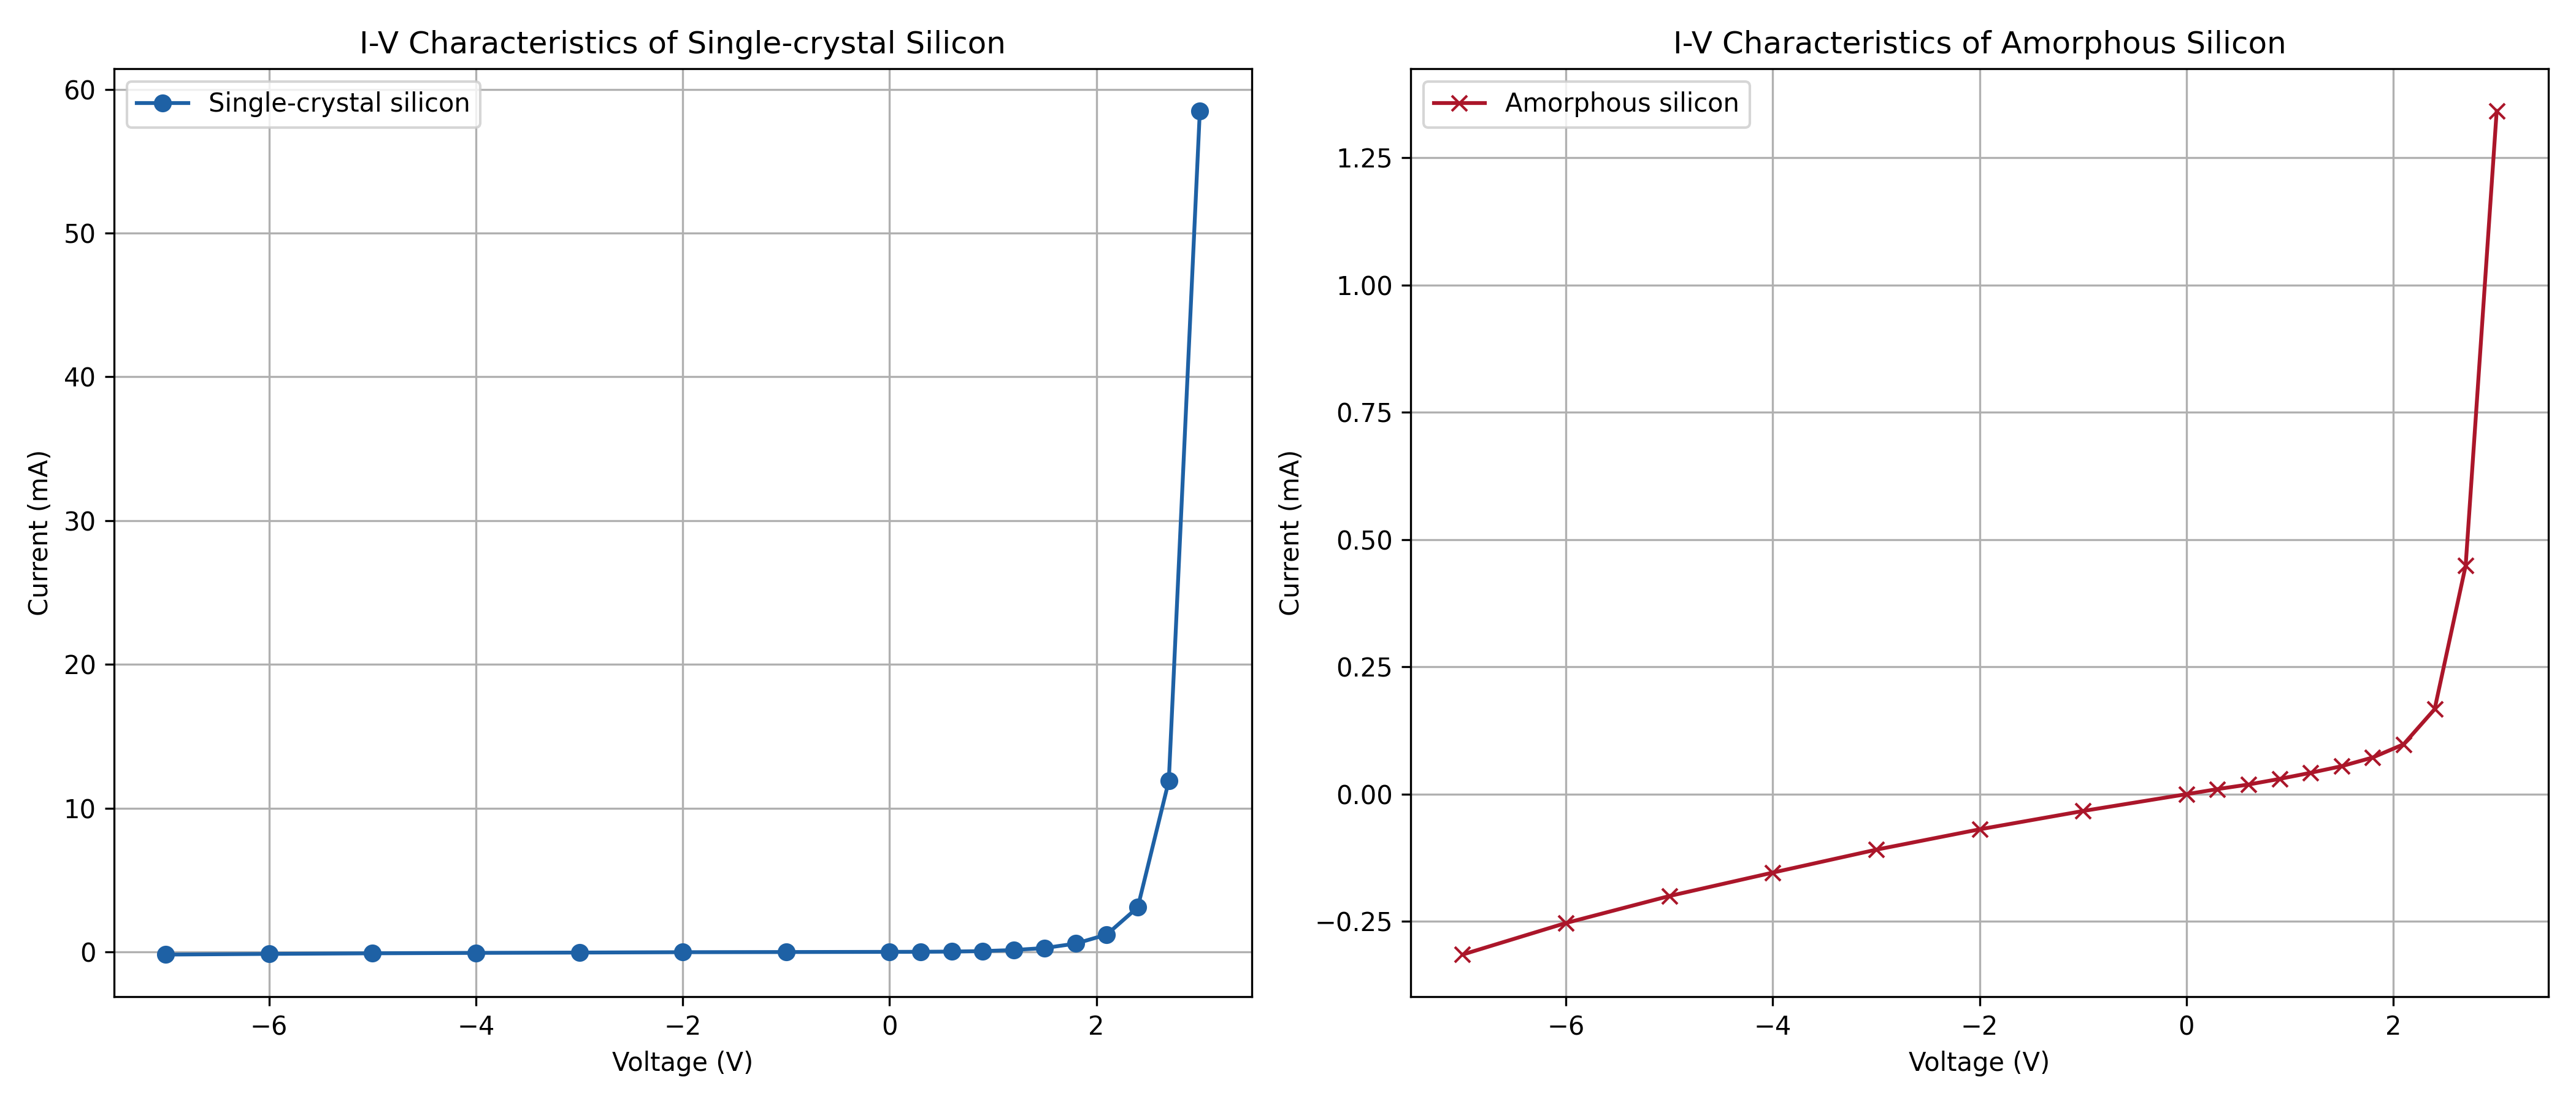
\includegraphics[width=0.8\textwidth]{1.png}
\end{figure}

\subsection{根据表2数据,画出两种太阳能电池的开路电压随光强变化的关系曲线以及短路电流随光强变化的关系曲线。}

\begin{figure}[!htbp]
    \centering
    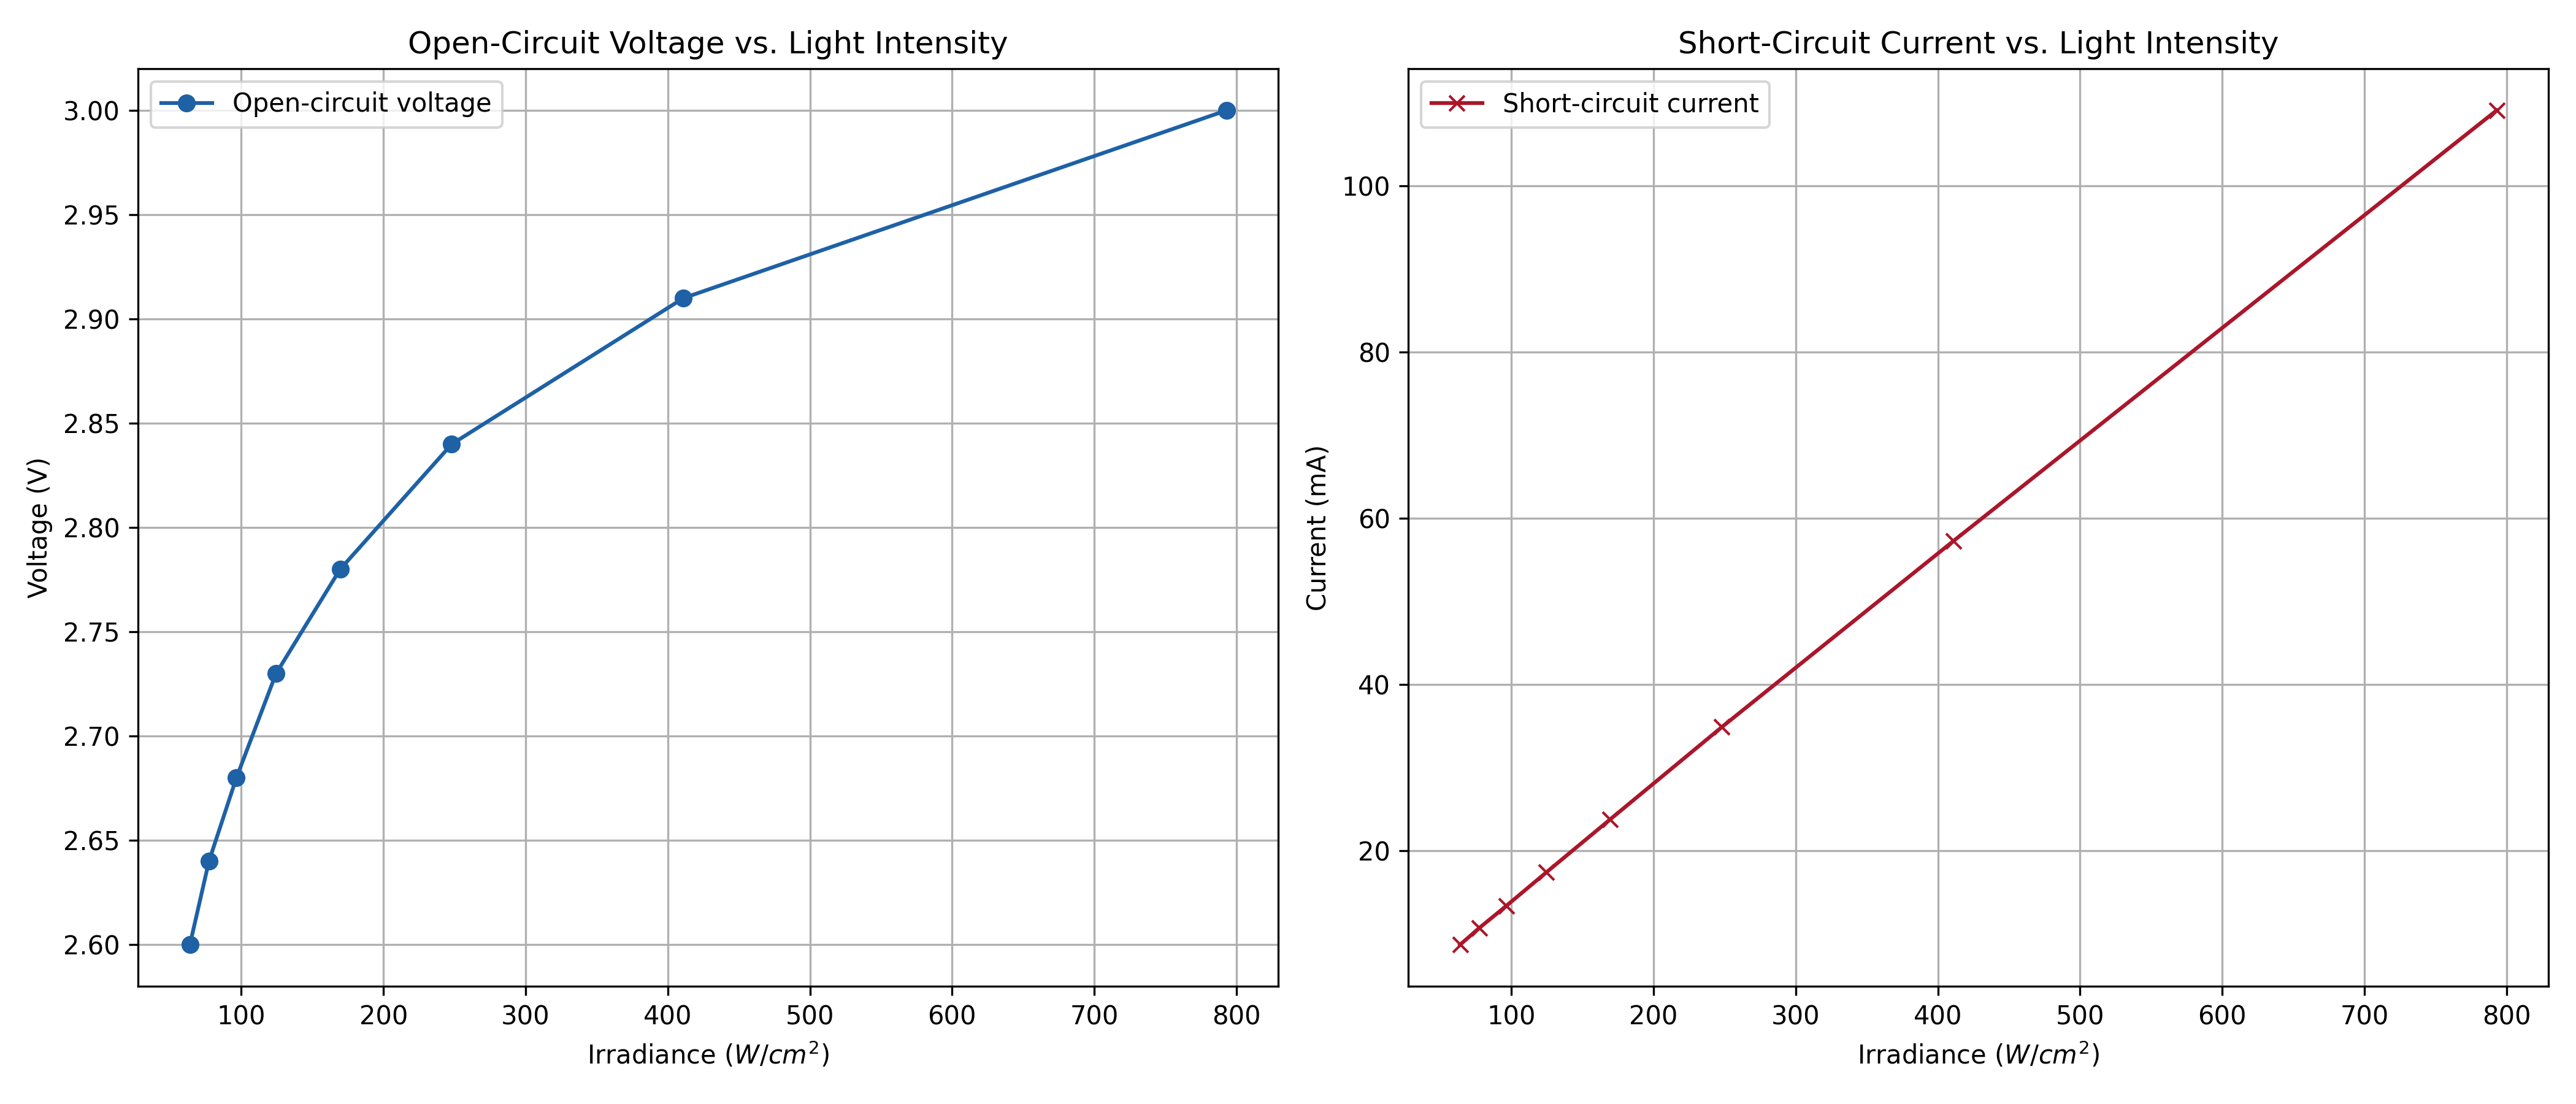
\includegraphics[width=0.8\textwidth]{2_0.png}
    \caption{单晶硅开路电压/短路电流与光强关系曲线}
\end{figure}

\begin{figure}[!htbp]
    \centering
    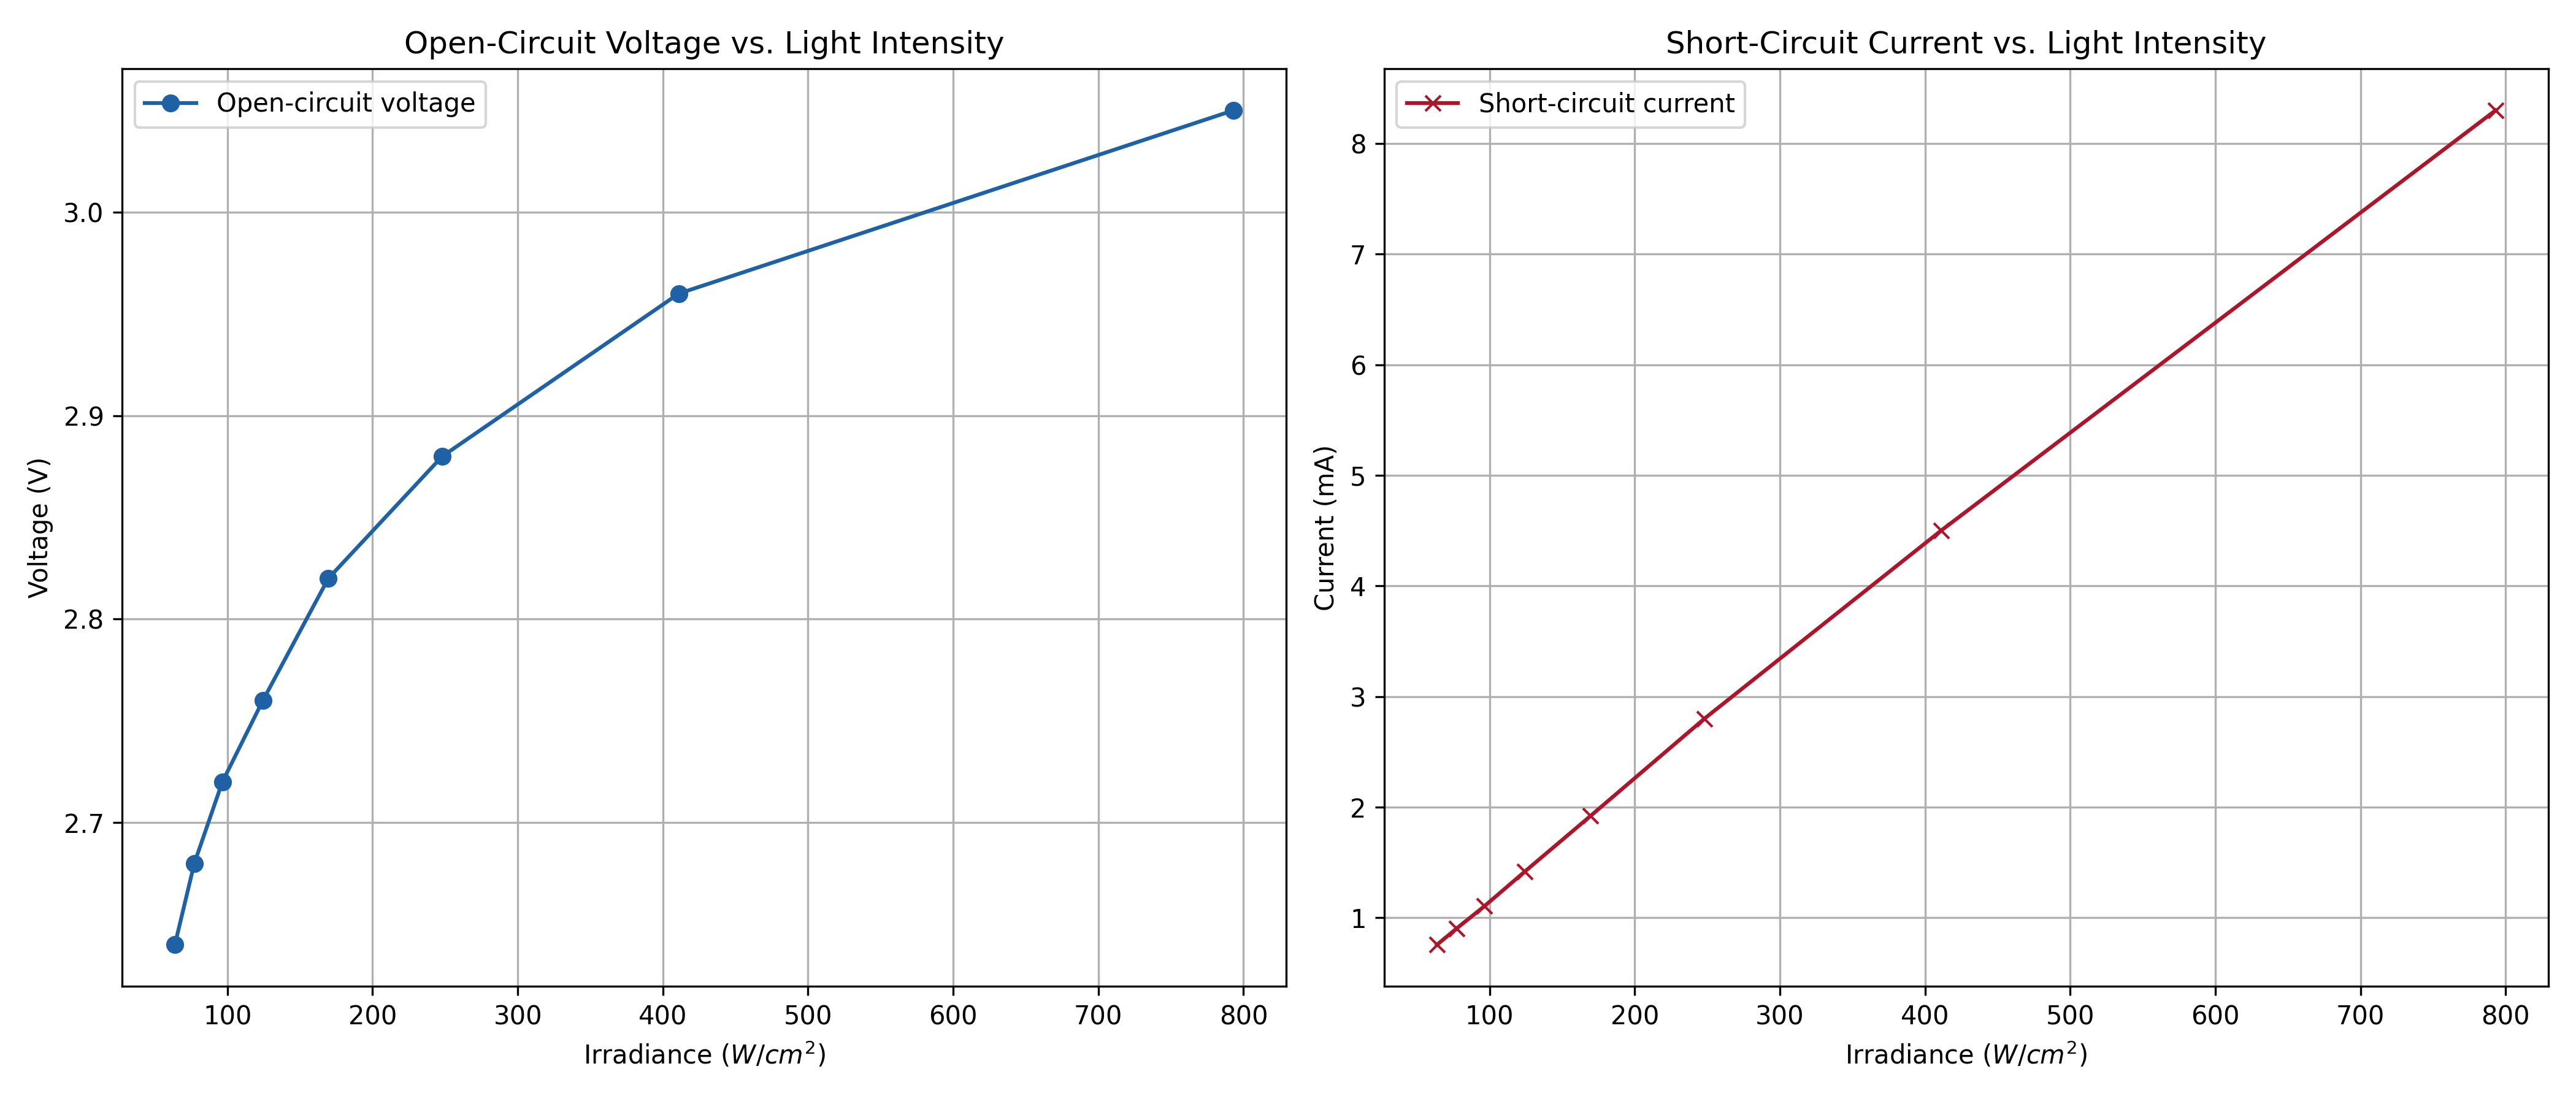
\includegraphics[width=0.8\textwidth]{2_1.png}
    \caption{非晶硅开路电压/短路电流与光强关系曲线}
\end{figure}

\subsection{根据表3数据作两种太阳能电池的输出伏安特性曲线及功率曲线。计算最大功率$P_{max}$和最佳匹配负载电阻。}

\begin{figure}[!htbp]
    \centering
    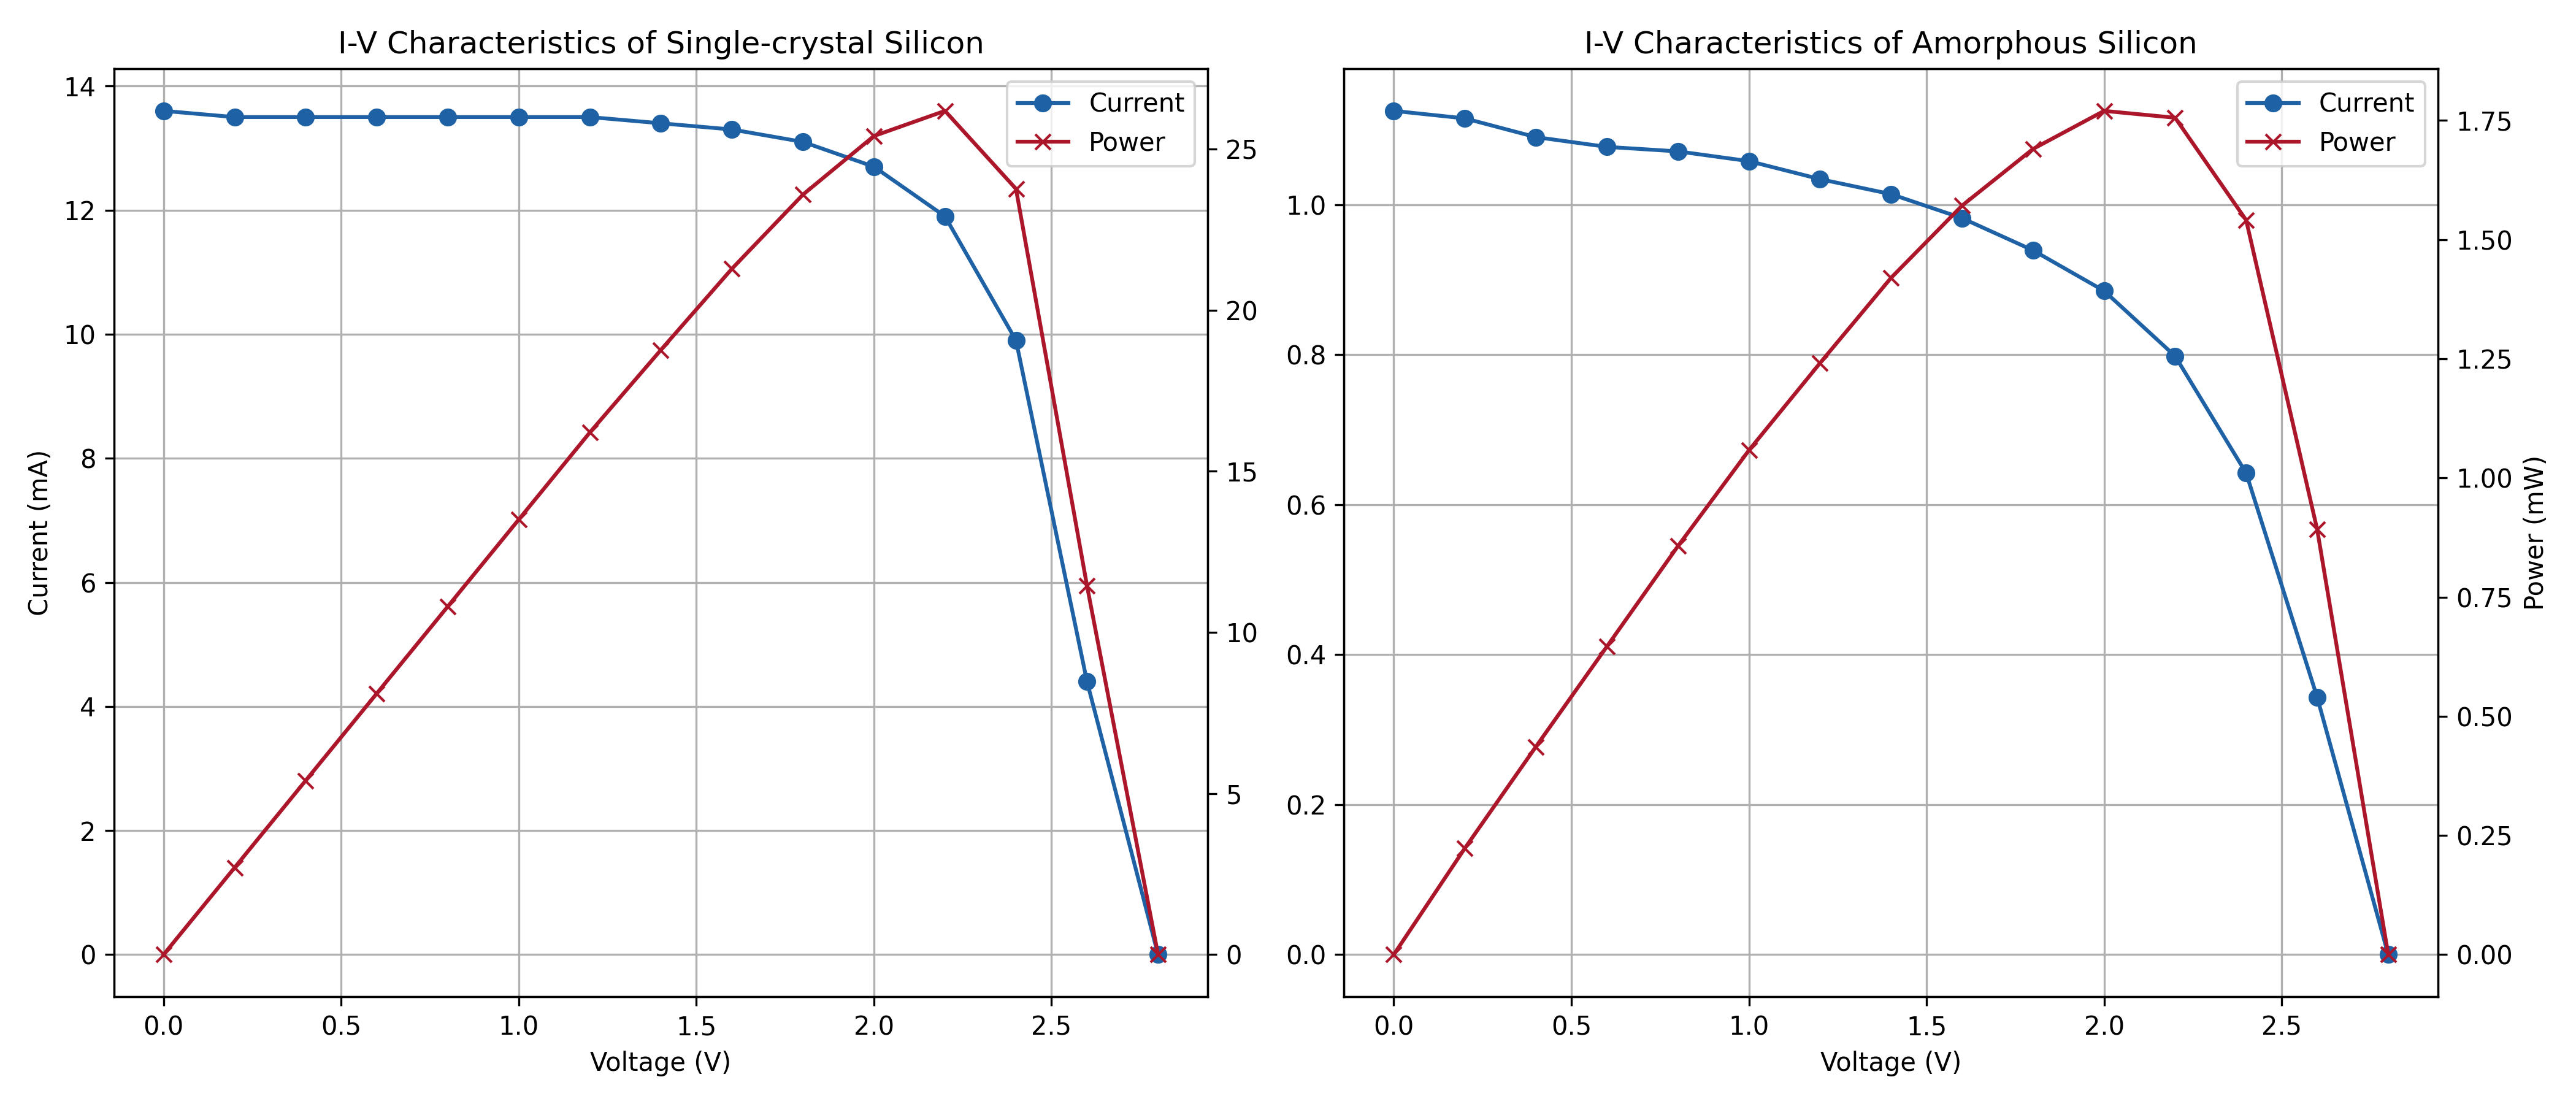
\includegraphics[width=0.8\textwidth]{3.png}
    \caption{伏安特性曲线及功率曲线}
    \label{fig:output_characteristics_and_power_curve_of_monocrystalline_silicon}
\end{figure}

单晶硅在$ U = 2.2 v , I = 11.9 mA $ 时,功率最大,为$ P_{max} = 26.18 mW $,最佳匹配负载电阻为$ R_{m} = 184.87 \Omega $。

非晶硅在$ U = 2.0 v , I = 0.885 mA $ 时,功率最大,为$ P_{max} = 1.77 mW $,最佳匹配负载电阻为$ R_{m} = 2262.71 \Omega $。

\subsection{根据表3数据计算两种太阳能电池的填充因子和转换效率。转换效率为:$$ \eta = \frac{P_{max}}{P_{m}} = \frac{P_{max}}{SI} $$其中S为太阳能电池面积(按50mm*50mm计算),I为光强。}

此处光强为$ 96.4 W/m^2 $,太阳能电池面积为$ 50 mm * 50 mm = 0.0025 m^2 $,则有:

$$ \eta_{sig} = \frac{P_max}{SI} = 10.86\% \quad \eta_{amo} = \frac{P_max}{SI} = 0.73\% $$

填充因子为:

$$ FF_{sig} = \frac{P_{max}}{V_{oc}I_{sc}} = 68.75\% \quad FF_{amo} = \frac{P_{max}}{V_{oc}I_{sc}} = 56.19\% $$

\subsection{分析可能的误差来源。}

测量设备如电压和电流传感器的精度可能导致误差,设备校准不准确会影响结果。其次,环境条件如光强波动和温度变化也会影响太阳能电池的性能,导致测量结果不一致。此外,实验操作中的接触不良或测试时间控制不当,材料均匀性差异,局部遮挡或照射不均匀等也会引发误差。通过改进设备校准、控制实验条件、以及减少材料缺陷,可以有效降低这些误差的影响。

\end{document}